% kapitel5.tex
\chapter{Optimization Studies for the Event Selection}

\section{Search for Discriminating Variables }
\label{distributions}
The first part of the optimization studies is the search for variables which provide a significant distinction between background and signal.
Caused by the basic selection discussed in section \ref{basic selection} there is already much background rejected.
Moreover the requirement of two large-R jets cause that the remaining background events contain high energies, because large-R jets, which fulfill the minimum criteria, have to be produced.
This complicates the search for discriminating variables, because the signal is expected to contain high energies,too.\\
Figure \ref{H_T} shows the distribution for the scalar sum of the transverse momenta of all jets in an event.

\begin{figure}
\centering
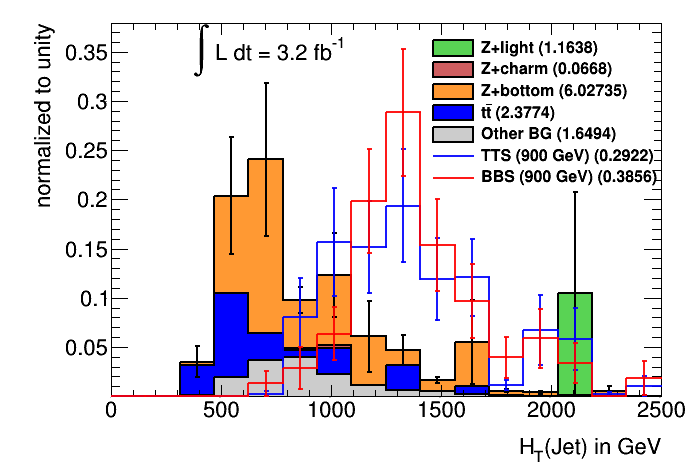
\includegraphics[width=8cm]{figures/H_T.png}
\caption{Plot for the scalar sum of all jet $p_{T}$'s in an event after the preselection. 
Both signal and background are presented and the distributions are normalized to unity. 
The weighted number of events is displayed in the legend in brackets next to the processes. 
The number of events are expected for a integrated luminosity $\int L dt$ = \SI{3.2}{fb^{-1}}}
\label{H_T}
\end{figure}

The distribution shows, that the signal is shifted to the right compared to the background, because there is more energy in the events resulting from the very massive vector-like quarks. 
Figure \ref{Zpt} presents the distribution of the Z candidate $p_{T}$.
\begin{figure}
\centering
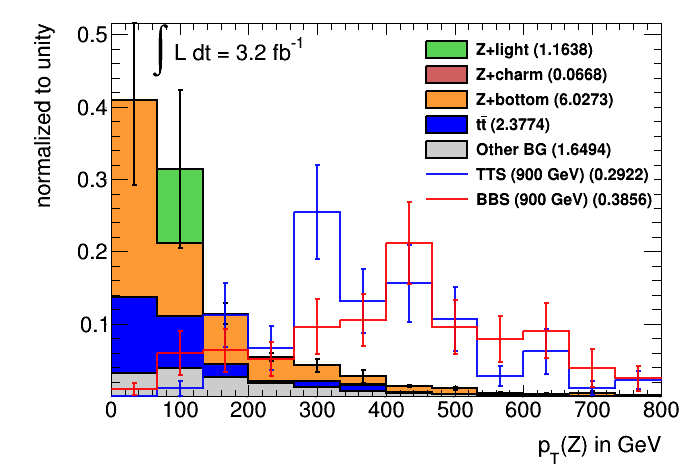
\includegraphics[width=8cm]{figures/Zpt.png}
\caption{Plot for the Z candidate $p_{T}$. 
Both signal and background are presented and the distributions are normalized to unity. 
The weighted number of events is displayed in the legend in brackets next to the processes. 
The number of events are expected for a integrated luminosity $\int L dt$ = \SI{3.2}{fb^{-1}}}
\label{Zpt}
\end{figure}

As mentioned for the $H_{T}$-distribution the signal is shifted to the right. That is as expeced, because the Z candidate results straight from the vector-like quark and should have a $p_{T}$ about \SI{450}{GeV}.
In figure \ref{leadingljet} the $p_{T}$ of the leading large-R jet is represented, which means the $p_{T}$ of the large-R jets with the highest $p_{T}$ in an event.
\vspace{-0.5cm}
\begin{figure}[h!]
\centering
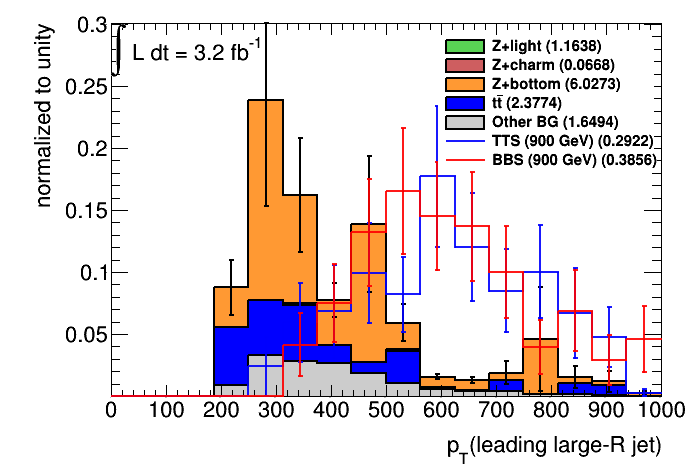
\includegraphics[width=8cm]{figures/leadingljet.png}
\caption{Plot for the leading large-R jet $p_{T}$. 
Both signal and background are presented and the distributions are normalized to unity. 
The weighted number of events is displayed in the legend in brackets next to the processes. 
The number of events are expected for a integrated luminosity $\int L dt$ = \SI{3.2}{fb^{-1}}.}
\label{leadingljet}
\end{figure}

In the plot also a shift of the signal to the right is visible.
Figure \ref{mZb+mZt} shows the distribution of the invariant mass of the Z candidate and the highest $p_{T}$ b-jet and \ref{mZt} the invariant mass of the Z candidate and the highest $p_{T}$ top-jet.


%\resizebox{0.48\columnwidth}{!}{
\begin{figure}[h]
    \centering
    \resizebox{0.46\columnwidth}{!}{
    \begin{subfigure}{.49\textwidth}
      \centering
      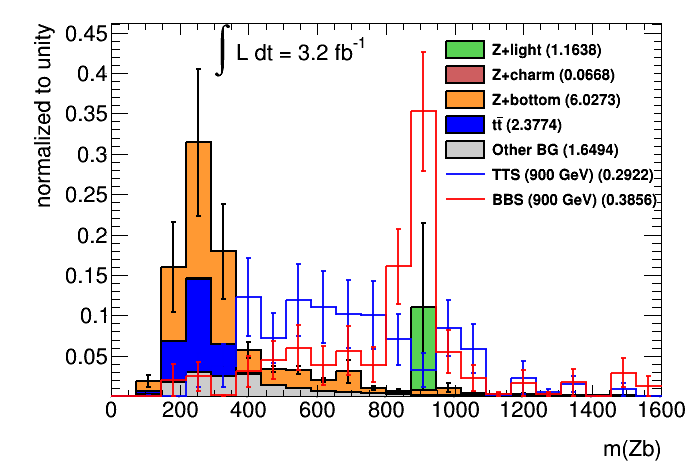
\includegraphics[width=.99\linewidth]{figures/mZb.png}
      \caption{}
      \label{mZbdist}
    \end{subfigure}
    }
    \resizebox{0.46\columnwidth}{!}{
    \begin{subfigure}{.49\textwidth}
      \centering
      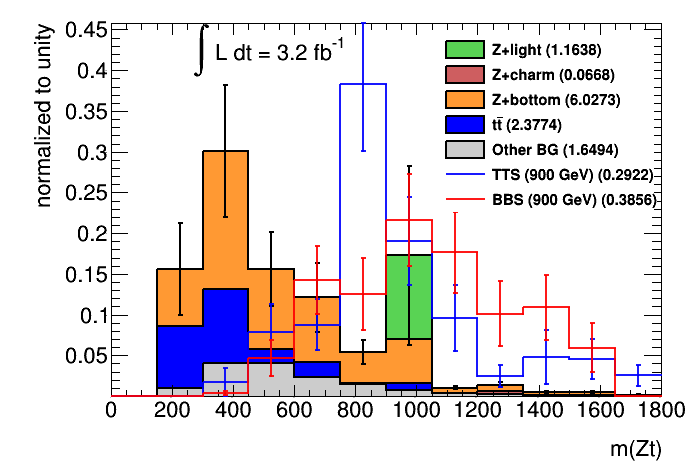
\includegraphics[width=.99\linewidth]{figures/mZt.png}
      \caption{}
      \label{mZtdist}
    \end{subfigure}
    }
    \caption{Plot for the invariant mass of the Z candidate and the highest $p_{T}$ b-jet (a) and the invariant mass of the Z candidate and the highest $p_{T}$ top-jet (b)  . 
Both signal and background are presented and the distributions are normalized to unity. 
The weighted number of events is displayed in the legend in brackets next to the processes. 
The number of events are expected for a integrated luminosity $\int L dt$ = \SI{3.2}{fb^{-1}}.}
    \label{mZb+mZt}   
\end{figure}
%}
The signal is shifted to the right caused by the same argumentation mentioned before. 
For the BBS signal process there is a peak at \SI{900}{GeV} in figure \ref{mZbdist}.
This is as expected because the Z candidate and the highest $p_{T}$ b-jet should result from the vector-like quark decay B \texorpdfstring{$\longrightarrow$}~Zb.
The peak of the TTS signal in figure  \ref{mZtdist} also results from a vector-like quarks decay T \texorpdfstring{$\longrightarrow$}~Zt, therefore the peak at \SI{900}{GeV} is also as expected.\\
Generally the presented distributions provide the possobility to achieve a distinction between background and signal by requiring limits for different variables.


\section{Significance for Different Cuts}
In this section the significance for different limits on variables, which are shown in section \ref{distributions}, are examined.
As used in previous analysis \cite{8tevanalysis} $m(Zb)$ is chosen as final discriminant for the BBS process, but in this analysis $m(Zt)$ is chosen sepeatly for the TTS process.
Boosted analysis provide the possibility of this variable by using the top-tag.
The optimization studys are performed concering an interval of the final discriminat distributions.
The interval is chosen, starting from the highest values of $m(Zb)$ and $m(Zt)$ until 80\% of all signal events of BBS and TTS are within the interval.
This interval is chosen because the signal is shifted to higher values of $m(Zb)$ and $m(Zt)$.
Therefore the in the interval the main background is rejected. 
The significance of the signal relative to the fluctuations of the background is investigated with formula $\frac{s}{\sqrt{b}}$, while $\sqrt{b}$ describes the statistical uncertainty of the background and $s$ the number of signal events.
Figure \ref{mZbcut} and \ref{mZtcut} show the significance as function of varying limits considering the vaiables presented in section \ref{distributions} for $m(Zb)$ and $m(Zt)$. 
\begin{figure}[h]
    \centering
    \resizebox{0.46\columnwidth}{!}{
    \begin{subfigure}{.49\textwidth}
      \centering
      \includegraphics[width=.99\linewidth]{figures/H_TcutmZb.pdf}
      \caption{}
      \label{mZb}
    \end{subfigure}
    }
    \resizebox{0.46\columnwidth}{!}{
    \begin{subfigure}{.49\textwidth}
      \centering
      \includegraphics[width=.99\linewidth]{figures/H_TcutmZt.pdf}
      \caption{}
      \label{mZb}
    \end{subfigure}
    }
    \resizebox{0.46\columnwidth}{!}{
    \begin{subfigure}{.49\textwidth}
      \centering
      \includegraphics[width=.99\linewidth]{figures/leadingljetptcutmZb.pdf}
      \caption{}
      \label{mZt}
    \end{subfigure}
    }
    \resizebox{0.46\columnwidth}{!}{
    \begin{subfigure}{.49\textwidth}
      \centering
      \includegraphics[width=.99\linewidth]{figures/leadingljetptcutmZt.pdf}
      \caption{}
      \label{mZt}
    \end{subfigure}
    }
    \resizebox{0.46\columnwidth}{!}{
    \begin{subfigure}{.49\textwidth}
      \centering
      \includegraphics[width=.99\linewidth]{figures/ZptcutmZb.pdf}
      \caption{}
      \label{mZt}
    \end{subfigure}
    }
     \resizebox{0.46\columnwidth}{!}{
    \begin{subfigure}{.49\textwidth}
      \centering
      \includegraphics[width=.99\linewidth]{figures/ZptcutmZt.pdf}
      \caption{}
      \label{mZt}
    \end{subfigure}
    }
    \caption{Plot for the significance for m(Zb) as function of varying limits for $H_{T}$ (a), leading large-R jet $p_{T}$ and Z boson $p_{T}$.
    The values of the limits varying with \SI{50}{GeV} steps.}
    \label{mZbcut}   
\end{figure}

The graphs are consistent with the distributions for the different variables, because the trend is as expected by regarding the distributions in section \ref{distributions}.
For $H_{T}$ and leading large-R jet $p_{T}$ the significance has higher values for lower limits and decreases fastly for higher limits.
This is as expected, because the signal distribution is only slighly shifted to higher values and therefore for higher limits the peak of the signal is rejected.
For the Z candidate $p_{T}$ distribution the distinction between background and signal is more significant.
Therfore higher limits can be set to reject a lot of background and do not cut into the main signal region.










\section{Proposel for a Boosted Event Selection}

